\section{User Interface Design}

The design of the web application will use the Google Material UI elements to give out a more native look on
Android Devices, which we expect to be the majority of our user base.
The design of the native applications will, instead, comply with the target platform. This process will be handled
by the framework (e.g. Ionic framework) we'll use to port the Web App to Android and iOS.

In the following pages some mock ups are provided with a description of how the user will interact with them.
\newpage

\subsection{User Registration}
\begin{figure}[H]
  \centering
  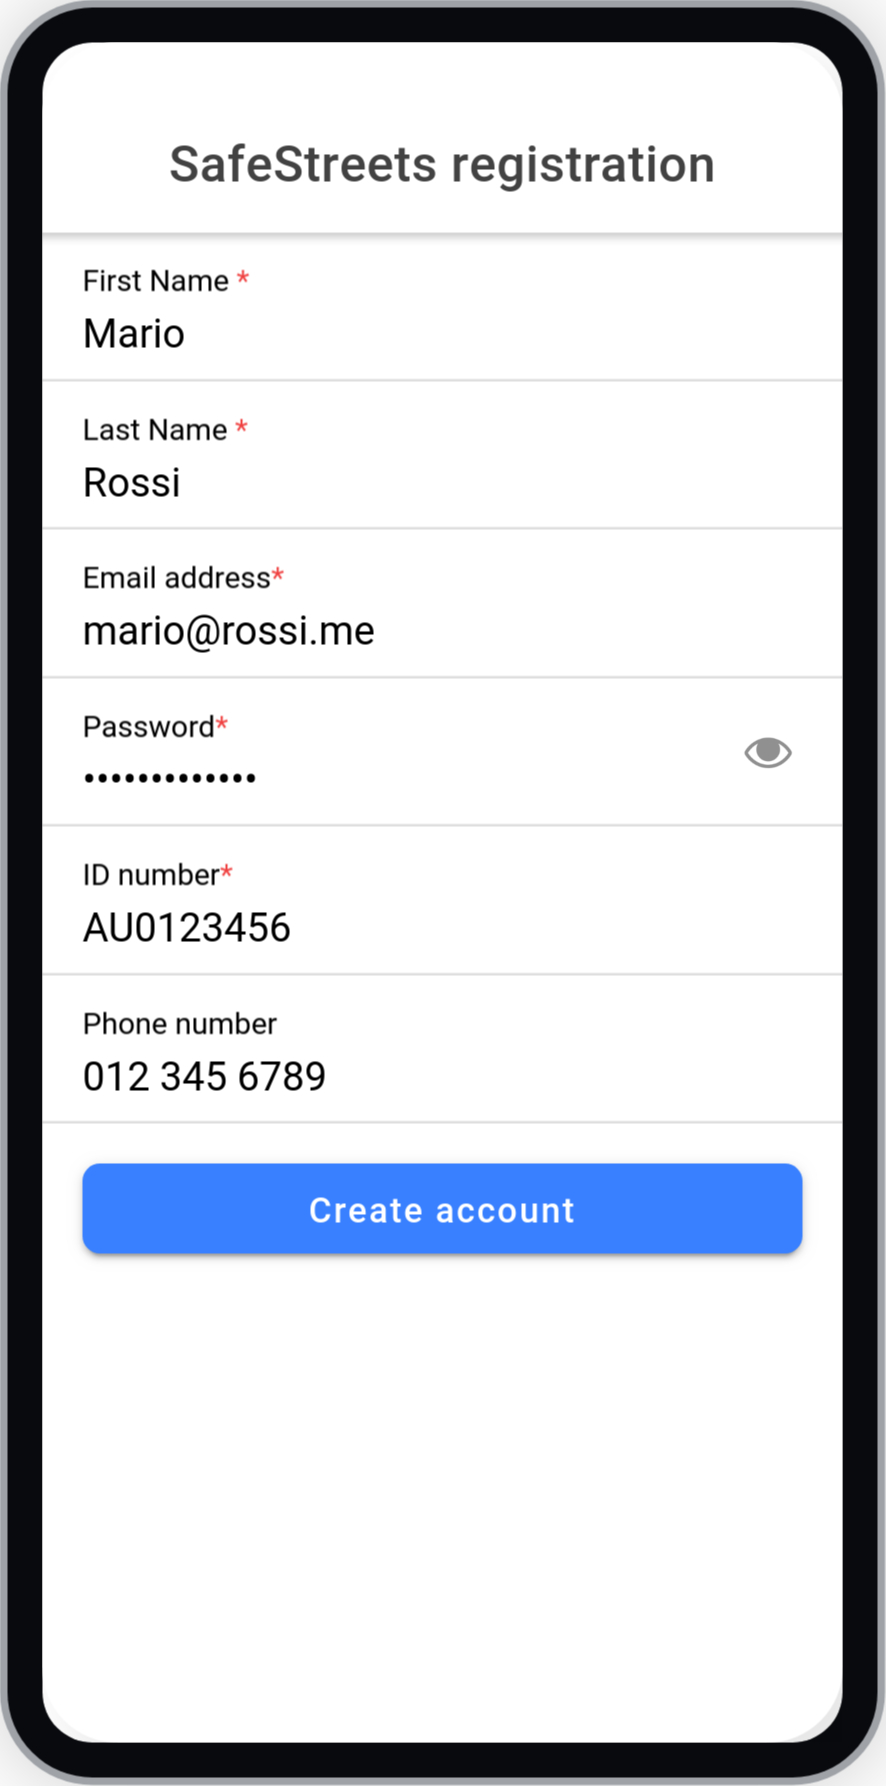
\includegraphics[origin=c,width=\textwidth,height=.90\textheight,keepaspectratio]{DD_Images/UserInterface/Registration.jpg}
  \caption{\textit{User Registration}}
\end{figure}

The registration process asks the user for personal information about who they are and require them to enter
their identification number.
\subsection{User Login}
\begin{figure}[H]
  \centering
  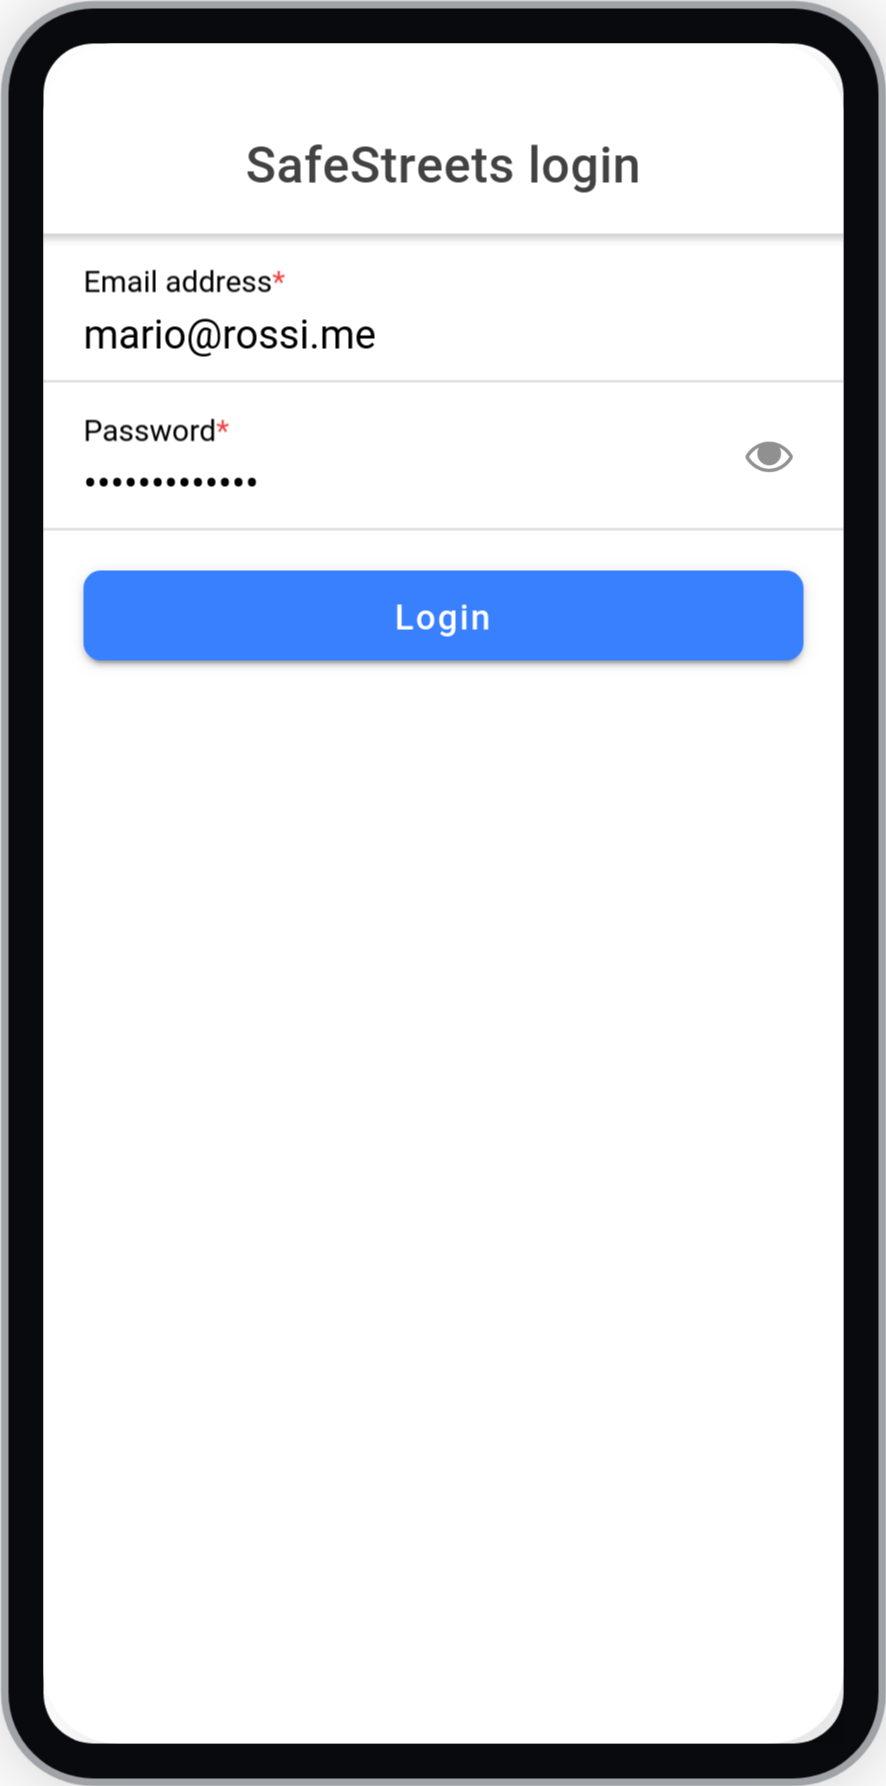
\includegraphics[origin=c,width=\textwidth,height=.70\textheight,keepaspectratio]{DD_Images/UserInterface/Login.jpg}
  \caption{\textit{User Login}}
\end{figure}

The login phase asks for the email and the previously selected password like a common login process.
\subsection{Report a Violation}
\begin{figure}[H]
  \centering
  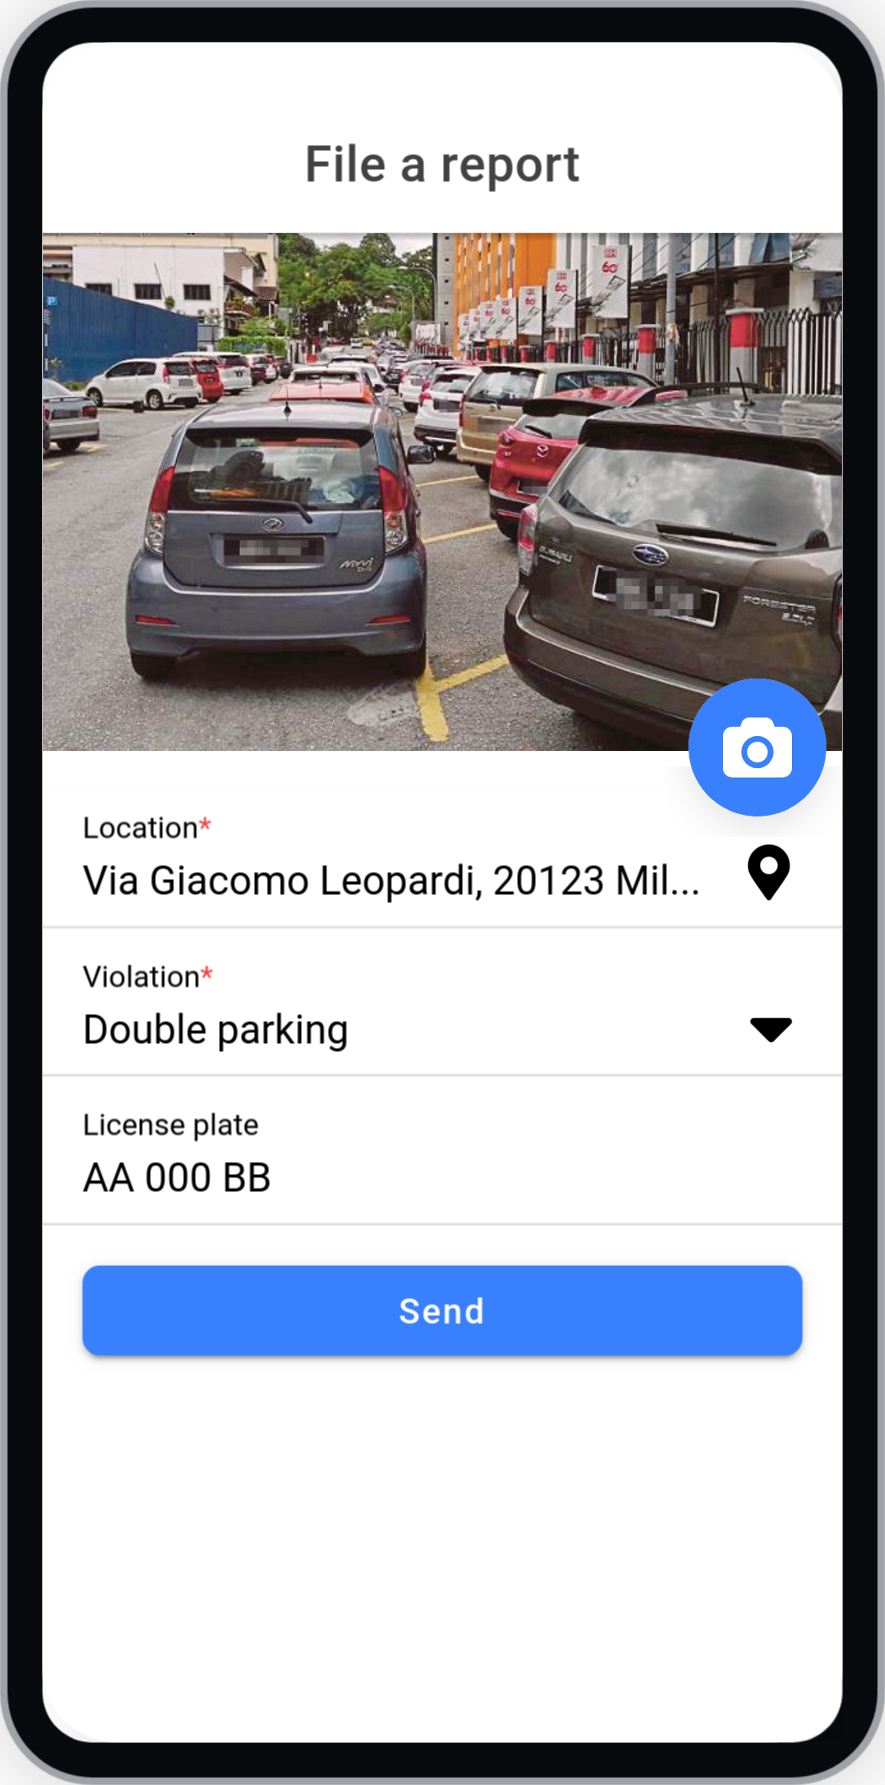
\includegraphics[origin=c,width=\textwidth,height=.70\textheight,keepaspectratio]{DD_Images/UserInterface/Report.jpg}
  \caption{\textit{Report a Violation}}
\end{figure}

In this mock up it can be seen that the user is required to insert images regarding the violation they want to report,
the location where the violation happened and the category of violation identified.
Optionally the user can add a license plate to ease the verification process.
\subsection{Report Validation}
\begin{figure}[H]
  \centering
  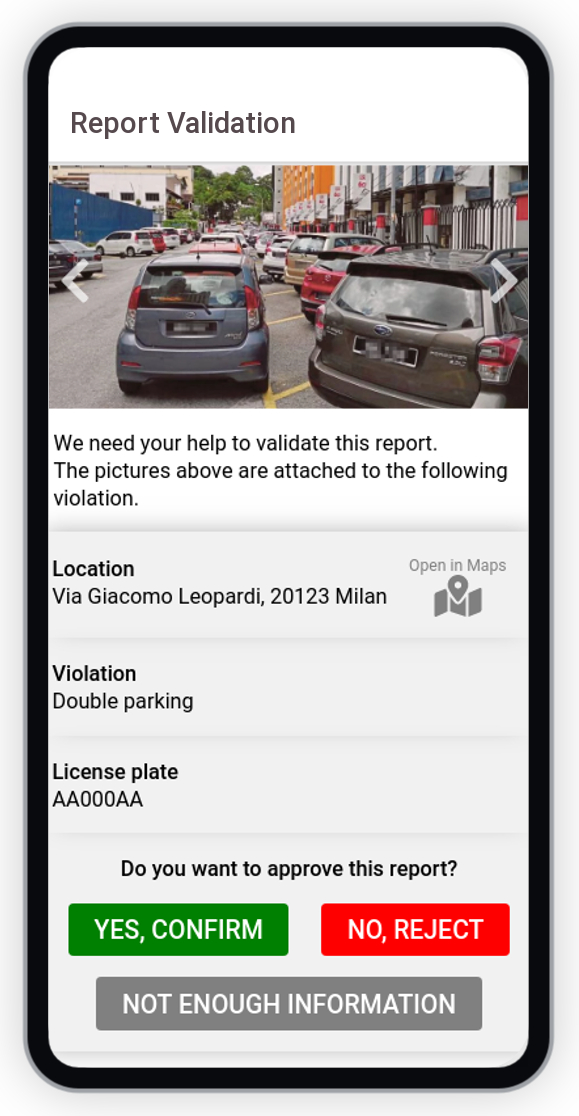
\includegraphics[origin=c,width=\textwidth,height=.70\textheight,keepaspectratio]{DD_Images/UserInterface/Validation.jpg}
  \caption{\textit{Report Validation}}
\end{figure}

Reports are validated by the community, so every time a new violation is submitted to SafeStreets some users will be notified and will see this screen.
The report is anonymous, so the users that validate it don't see who sent it, but only the relevant details about the notified infraction. 
The user is therefore asked to click one of the three buttons to either validate, reject or ignore the report.
\subsection{Prize Catalog}
\begin{figure}[H]
  \centering
  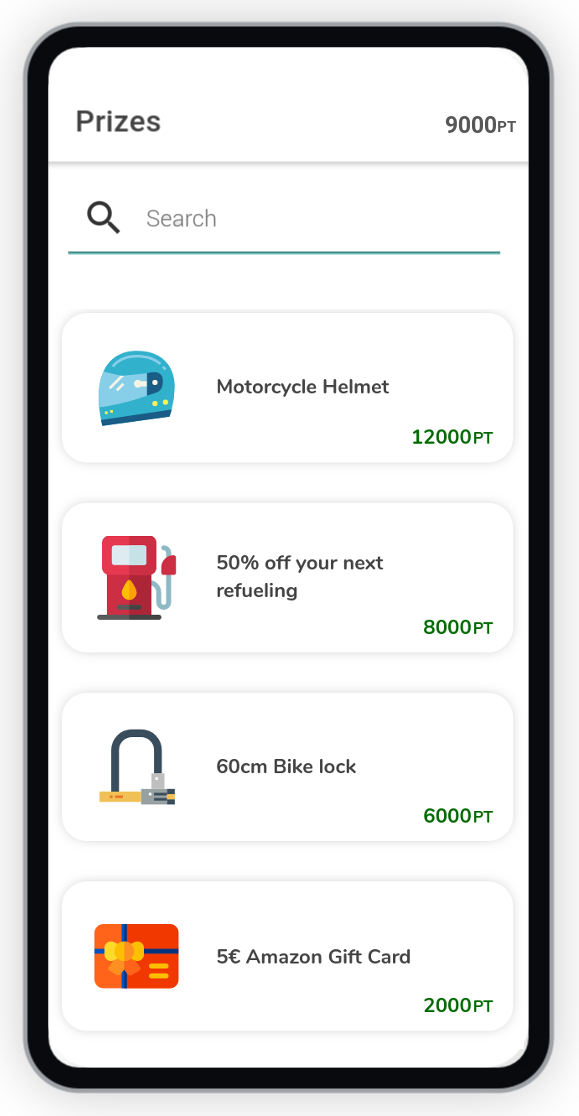
\includegraphics[origin=c,width=\textwidth,height=.70\textheight,keepaspectratio]{DD_Images/UserInterface/Catalog.jpg}
  \caption{\textit{Prize Catalog}}
\end{figure}

Prizes are an incentive for users to use the application. Users can be assigned points when they file or evaluate a report.
In the mock up above some example of rewards are provided. Prizes, being an addendum to the platform,
will be provided to our users by external partners.
\subsection{UX Design}
\begin{figure}[H]
  \centering
  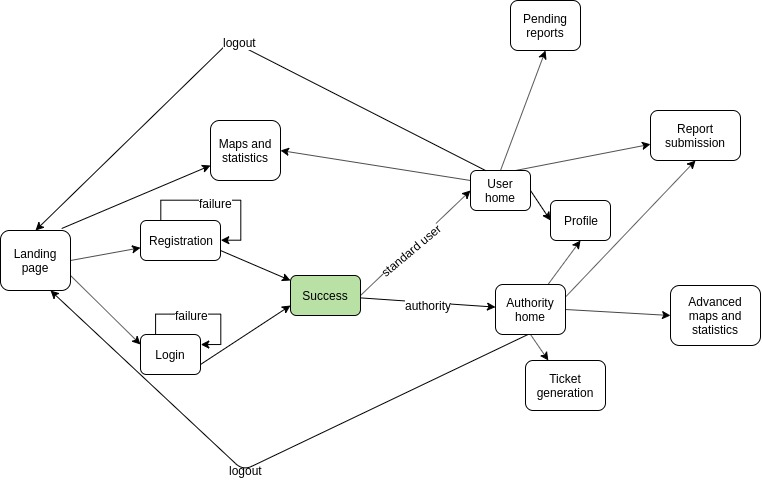
\includegraphics[origin=c,width=\textwidth,height=.70\textheight,keepaspectratio]{DD_Images/UserInterface/UXDiagram.jpg}
  \caption{\textit{UX Diagram}}
\end{figure}

The diagram above displays the interaction between the different views for both a standard user and an authority.
